\documentclass[11pt]{exam}
\usepackage[brazil]{babel}
\usepackage{graphicx}
\usepackage{geometry}
\usepackage{amssymb, amsfonts, amsmath}
\usepackage[svgnames]{xcolor}
\usepackage{tcolorbox}
\usepackage[utf8]{inputenc}
\usepackage{lmodern}
\usepackage{indentfirst}
\usepackage{microtype}
\usepackage[brazil]{babel}
\usepackage{parskip}

% -- question choice correct align
\usepackage{xpatch}
\xpatchcmd{\oneparchoices}{\penalty -50\hskip 1em plus 1em\relax}{\hfill}{}{}
\xpatchcmd{\oneparchoices}{\penalty -50\hskip 1em plus 1em\relax}{\hfill}{}{}

\renewcommand\choicelabel{(\alph{choice})}
\begin{document}

% .. capa

\definecolor{titlepagecolor}{HTML}{F6D5A8}
\begin{titlepage}
  \newgeometry{left=7.5cm}
  \pagecolor{titlepagecolor}
  \noindent
  \makebox[0pt][l]{\rule{1.9\textwidth}{1pt}}
  \par
  \noindent
  \textbf{{\huge{Lista de Exercício com Resolução}}}
  \vfill
  \noindent
  {\huge Progressão Aritmética e Geométrica}
  \vskip\baselineskip
  \noindent
  \Large{Dezembro, 2021}
\end{titlepage}

\nopagecolor

\section*{Fundamentos - P.A}

\begin{questions}
  \question Determine $x$ de modo que $(x ; 2x + 1 ; 5x + 7)$ seja uma P.A.

  \vspace{0.5cm}

  \question Obtenha 3 números em P.A, de modo que a soma entre esses seja igual a 3 e a soma de seus quadrados seja 11

  \vspace{0.5cm}

  \question Os números que exprimem o lado, a diagonal e a área de um quadrado estão, respectivamente, em P.A. Determine quanto mede o lado.

  \vspace{0.5cm}

  \question Demonstre que se $(a, b, c)$ é uma P.A, então $(a^{2}bc, ab^{2}c, abc^{2})$ também é.

  \vspace{0.5cm}

  \question Determine qual é o primeiro termo negativo da P.A $f = \{60, 53, 46, \dots\}$.

  \vspace{0.5cm}

  \question Sabe-se que $a_{10} = 7$ e que $a_{12} = -8$. Monte a P.A.

  \vspace{0.5cm}

  \question  De 100 a 1000, quanto são os múltiplos de 2 ou 3.

  \vspace{0.5cm}

  \question Obtenha a soma dos 200 primeiros termos da sequência dos números ímpares positivos. Cálcule também a soma dos $n$ primeiros termos iniciais dessa mesma sequência.

  \vspace{0.5cm}

  \question Um jardineiro tem que regar 60 roseiras plantadas ao longo de uma vereda retilínea e distando 1 m uma da outra. Ele enche seu regador numa fonte situada na mesma vereda, a 15 m da primeira roseira, e a cada viagem rega 3 roseiras. Começando e terminando na fonte, determine qual é o percurso total que ele terá que caminhar até regar todas as roseiras.

  \vspace{0.5cm}

  \question \textbf{(ITA-SP)} Considere a progressão aritmética ($a_{1}, a_{2}, a_{3}, \dots, a_{50}$) de razão $d$. Se $\displaystyle \sum_{n = 1}^{10} a_{n} = 10 + 25d$ e $\displaystyle \sum_{n = 1}^{50} = 4550$. Então $d - a_{1}$ é igual a:
  \vspace{0.4cm}

  \begin{oneparchoices}
    \choice 3
    \choice 6
    \choice 9
    \choice 11
    \choice 14
  \end{oneparchoices}

\end{questions}

\section*{Fundamentos - P.G}

\begin{questions}

  \question Prove que se $x, y, z$, nessa ordem, formam uma P.G, vale a relação

  \[(x + y + z)(x - y + z) = x^{2} + y^{2} + z^{2}\]

  \vspace{0.5cm}

  \question Os lados de um triângulo retângulo apresentam medidas em P.G. Determine o valor de $q$.

  \vspace{0.5cm}

  \question Dada uma P.G finita $(a_{1}, a_{2}, \dots, a_{10})$ onde $a_{1} = 2$ e $a_{2} = 6$, então determine se $(a_{10})^{\frac{1}{8}} = 3\cdot (2)^{\frac{1}{8}}$ é uma sentença verídica.

  \vspace{0.5cm}

  \question Prove que se $(a_{1}, a_{2}, a_{3}, \dots)$ é P.G, então $\displaystyle \left(\frac{1}{a_{1}}, \dots\right)$ também é.

  \vspace{0.5cm}

  \question Determine $\displaystyle \sum_{i = 3}^{n} 2^{i} = 4088$

  \vspace{0.5cm}

  \question Sabendo que $0 < q < 1$, calcule o valor da expressão da P.G infinita

  \[q + 2q^{2} + 3q^{3} + \dots\]

  \question \textbf{(IME–RJ)} Uma placa metálica com base $b$ e altura $h$ sofre sucessivas reduções da sua área, em função da realização de diversos cortes, conforme ilustrado na figura abaixo. A cada passo, a área à direita é removida e a placa sofre um novo corte. Determine a soma das áreas removidas da placa original após serem realizados $n$ cortes.

  \begin{center}
  \begin{figure}[ht]
    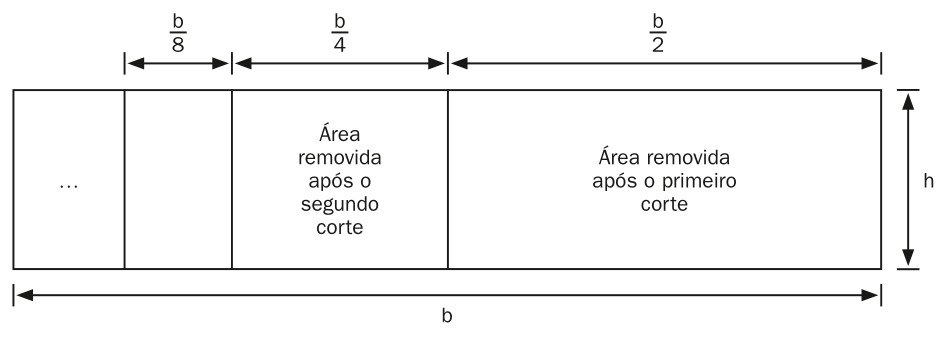
\includegraphics[width=12cm]{contents/ime-questao6}
    \centering
  \end{figure}
  \end{center}

  \question \textbf{(ITA-SP)} Seja $(a_{1}, a_{2}, \dots)$ uma progressão geométrica de razão $0 < a_{1} < 1$ e soma igual a $3a_{1}$. A soma dos três primeiros termos dessa progressão geométrica é igual a

  \vspace{0.3cm}

  \begin{oneparchoices}
    \choice $\displaystyle \frac{8}{27}$

    \choice $\displaystyle \frac{20}{27}$

    \choice $\displaystyle \frac{26}{27}$

    \choice $\displaystyle \frac{30}{27}$

    \choice $\displaystyle \frac{38}{27}$
  \end{oneparchoices}

  \vspace{0.5cm}

  \question \textbf{(Dep. de Matemática da Clínica Espiritual de Marabá - PA)} Para que os produtos dos termos da sequência

  \[\left(1, \sqrt{3}, \sqrt{3}^{2}, \sqrt{3}^{3}, \dots \sqrt{3}^{(n - 1)}\right)\]

  Seja igual a $3^{14}$, deverão ser consideradas, nessa sequência:

  \vspace{0.3cm}

  \begin{oneparchoices}
    \choice 8 termos
    \choice 6 termos
    \choice 10 termos
    \choice 9 termos
    \choice 7 termos
  \end{oneparchoices}

  \vspace{0.5cm}

  \question \textbf{(ITA-SP)} A progressão infinita $(a_{1}, \dots, a_{n}, \dots)$ tem razão $r < 0$. Sabe-se que a progressão infinita $(a_{1}, \dots, a_{(5n + 1)}, \dots)$ tem soma 8 e a progressão infinita $(a_{1}, \dots, a_{(5n)}, \dots)$ tem soma 2. Determine a soma da progressão $(a_{1}, \dots, a_{n}, \dots)$

\end{questions}

\pagebreak
\documentclass[11pt]{article}

\usepackage[svgnames]{xcolor}
\usepackage{tcolorbox}
\usepackage[utf8]{inputenc}
\usepackage{lmodern}
\usepackage{indentfirst}
\usepackage{microtype}
\usepackage{amsmath}
\usepackage[brazil]{babel}
\usepackage{parskip}
\usepackage[tmargin=1.5in, lmargin=1.25in, rmargin=1.25in, bmargin=1.0in]{geometry}

\title{Resolução da L.E (P.A e P.G)}
\author{Mickael Lima}
\date{Dezembro, 2021}

\begin{document}

\maketitle

\section{Progressão Aritmética}

\subsection{Fundamentos}

\subsubsection{Questão 1}

A questão lida com a formação básica de uma P.A. Para determinar o termo $x$ pedido, podemos igualar a constante de razão $r$ da seguinte forma:

\begin{tcolorbox}[colback=LightYellow]
\[(2x + 1) - x = (5x + 7) - (2x + 1)\]
\[x + 1 = 3x + 6\]
\[-2x = 5\]
\[x = -\frac{5}{2}\]
\end{tcolorbox}

A prova real é realizada substituíndo $x$ na sequência e verificando se de fato a mesma forma uma P.A com os três primeiros termos dados.

\begin{tcolorbox}[colback=LightYellow]
\[f = \left(-\frac{5}{2}, -2\cdot \frac{5}{2} + 1, -5\cdot \frac{5}{2} + 7 \right)\]
\[f = \left(-2.5, -4, -5.5\right)\]
\end{tcolorbox}

De fato, forma-se a P.A de $a_{1} = (-2.5)$ e $r = (-1.5)$.

\subsubsection{Questão 2}

O enunciado pede duas condições a ser cumpridas (além da formação em P.A)

\begin{itemize}
  \item A soma dos 3 números deve ser igual a 3
  \item A soma dos 3 números, cada um ao quadrado, deve ser igual a 11
\end{itemize}

Isso implica no seguinte sistema

\begin{tcolorbox}[colback=LightYellow]
\begin{equation*}
\begin{cases}
  (x - r) + x + (x + r) = 3 \\
  (x - r)^2 + x^2 + (x + r)^2 = 11 \\
\end{cases}
\end{equation*}
\end{tcolorbox}

Do primeiro membro, nota-se inicialmente que $r$ irá ser cancelado pela soma entre $-r$ e $+r$. Ficando apenas $3x = 3$. Desse modo, descobre-se $x = 1$. Jogando essa informação no segundo membro, poderemos manipular e descobrir $r$ efetivamente.

\begin{tcolorbox}[colback=LightYellow]
\[(1 - r)^{2} + 1 + (1 + r)^{2} = 11\]
\[(1^{2} - 2r + r^{2}) + 1 + (1^{2} + 2r + r^{2}) = 11\]
\end{tcolorbox}

\begin{tcolorbox}[colback=LightYellow]
\[3 + 2r^{2} = 11 \]
\[r = \pm 2\]
\end{tcolorbox}

Sendo $x = 1$ e $r = \pm 2$, podemos montar duas progressões aritméticas $f$ (para $r = 2$) e $g$ (para $r = -2$), como ilustrado abaixo.


\begin{tcolorbox}[colback=LightYellow]
  \[f = (-1, 1, 3)\]
  \[g = (3, 1, -1)\]

  \begin{itemize}
          \item Soma: $-1 + 1 + 3 = 3$
          \item Soma dos quadrados: $3^{2} + 1^{2} + (-1)^{2} = 11$
  \end{itemize}
\end{tcolorbox}

\subsubsection{Questão 3}

Chamaremos $l$ de lado, $d$ a diagonal e $a$ a área. Montemos a sequência $f = (l, d, a)$. Como o enunciado pede o valor algébrico de $l$, é interessante reescrever todos esses valores em função do mesmo. Utilizando os conhecimentos importados da Geometria Plana, podemos afirmar que a P.A terá a forma

\begin{tcolorbox}[colback=LightYellow]
\[f = (l, l\sqrt{2}, l^{2})\]
\end{tcolorbox}

A P.A se estabelecerá com a existência de $r$. Utilizando a mesma técnica da primeira questão, temos

\begin{tcolorbox}[colback=LightYellow]
\[l\sqrt{2} - l = l^{2} - l\sqrt{2} \]
\[l\sqrt{2} + l\sqrt{2} - l = l^{2}\]
\[2\cdot l\sqrt{2} - l = l^{2}\]
\[l = \frac{2\cdot l\sqrt{2} - l}{l}\]
\[l = \frac{2\cdot l\sqrt{2}}{l} - \frac{l}{l}\]
\[l = 2\sqrt{2} - 1\]
\end{tcolorbox}

\subsubsection{Questão 4}

\begin{tcolorbox}[colback=LightYellow]
\begin{itemize}
  \item Hipótese: $\Rightarrow f = (a, b, c)$ é uma P.A
  \item Tese: $\Rightarrow g = (a^{2}bc, ab^{2}c, abc^{2})$ é uma P.A
\end{itemize}
\end{tcolorbox}

A hipótese afirma que a sequência é, de fato, uma P.A. Isso permite-nos concluir que $b - a = c - b$. Se todos os 3 primeiros elementos forem multiplicados por $abc$, é necessário verificar se essa igualdade mantem-se juntamente com essa proporção. Na P.A da tese, tem-se

\[g = (a^{2}bc, ab^{2}c, abc^{2})\]

Supondo que ela, de fato, é uma P.A, a igualdade $ab^{2}c - a^{2}bc = abc^{2} - ab^{2}c$ é válida. No entanto, isso nada mais é que a igualdade da sequência $f$ multiplicada por $abc$ também. Outro modo de ver isso é considerar o seguinte:

\begin{tcolorbox}[colback=LightYellow]
\[ab^{2}c - a^{2}bc = abc(b - a)\]
\[abc^{2} - ab^{2}c = abc(c - b)\]
\end{tcolorbox}

O que mantem a mesma relação.

\subsubsection{Questão 5}

Temos inicialmente $a_{1} = 60$ e uma razão $r$ negativa igual a $-7$. Haverá o enésimo termo a qual $a_{n}$ ficará negativo, que pode ser ilustrado por $a_{n} = 60 + (n - 1)\cdot -7$. Fixaremos $a_{n} < 0$ e trabalharemos com essa inequação.

\[60 + (n - 1)\cdot -7 < 0\]
\[60 - 7n + 7 < 0\]
\[67 - 7n < 0\]
\[-7n < -67\]
\[n > \frac{67}{7} \approx 9.5\]

Como $n$ obrigatoriamente é um número inteiro, admitimos $n \geq 10$. Portanto, a sequência ficará negativa após o décimo termo. Isso é facilmente provado ao verificar $a_{10}$.

\[a_{10} = 60\cdot (9)\cdot -7 = (60 - 63) = (-3)\]
\end{document}

\end{document}
